\documentclass[a3paper, landscape]{article}
\usepackage[left=1cm, right=1cm, top=1cm, bottom=1cm]{geometry}
\usepackage[T2A]{fontenc}
\usepackage[utf8]{inputenc}
\usepackage[english]{babel}
\thispagestyle{empty}

\usepackage{tabularray}
\usepackage{tikz}
\usetikzlibrary{positioning, calc, tikzmark}
\addtocounter{figure}{3}

\newcommand{\tm}[2]{\tikzmarknode{#1}{#2}}

\tikzset{
    lnk/.style={thick},
    crd/.style={font=\scriptsize, fill=white, inner sep=1pt},
    ann/.style={font=\scriptsize},
}

\newcommand{\dbtable}[3]{%
    \node[inner sep=0pt, anchor=north] (#1) at (#2) {%
        \begin{tblr}{
            colspec = {Q[c,1.5em]Q[l,12em]},
            hline{1-3} = {solid},
            hline{Z} = {solid},
            vlines,
            rows = {font=\ttfamily\footnotesize, abovesep=2pt, belowsep=2pt},
            row{1} = {font=\bfseries\small, halign=c},
            column{1} = {font=\it\footnotesize, halign=c},
        }
            #3
        \end{tblr}%
    };%
}

\begin{document}
\begin{figure}[p]
\centering
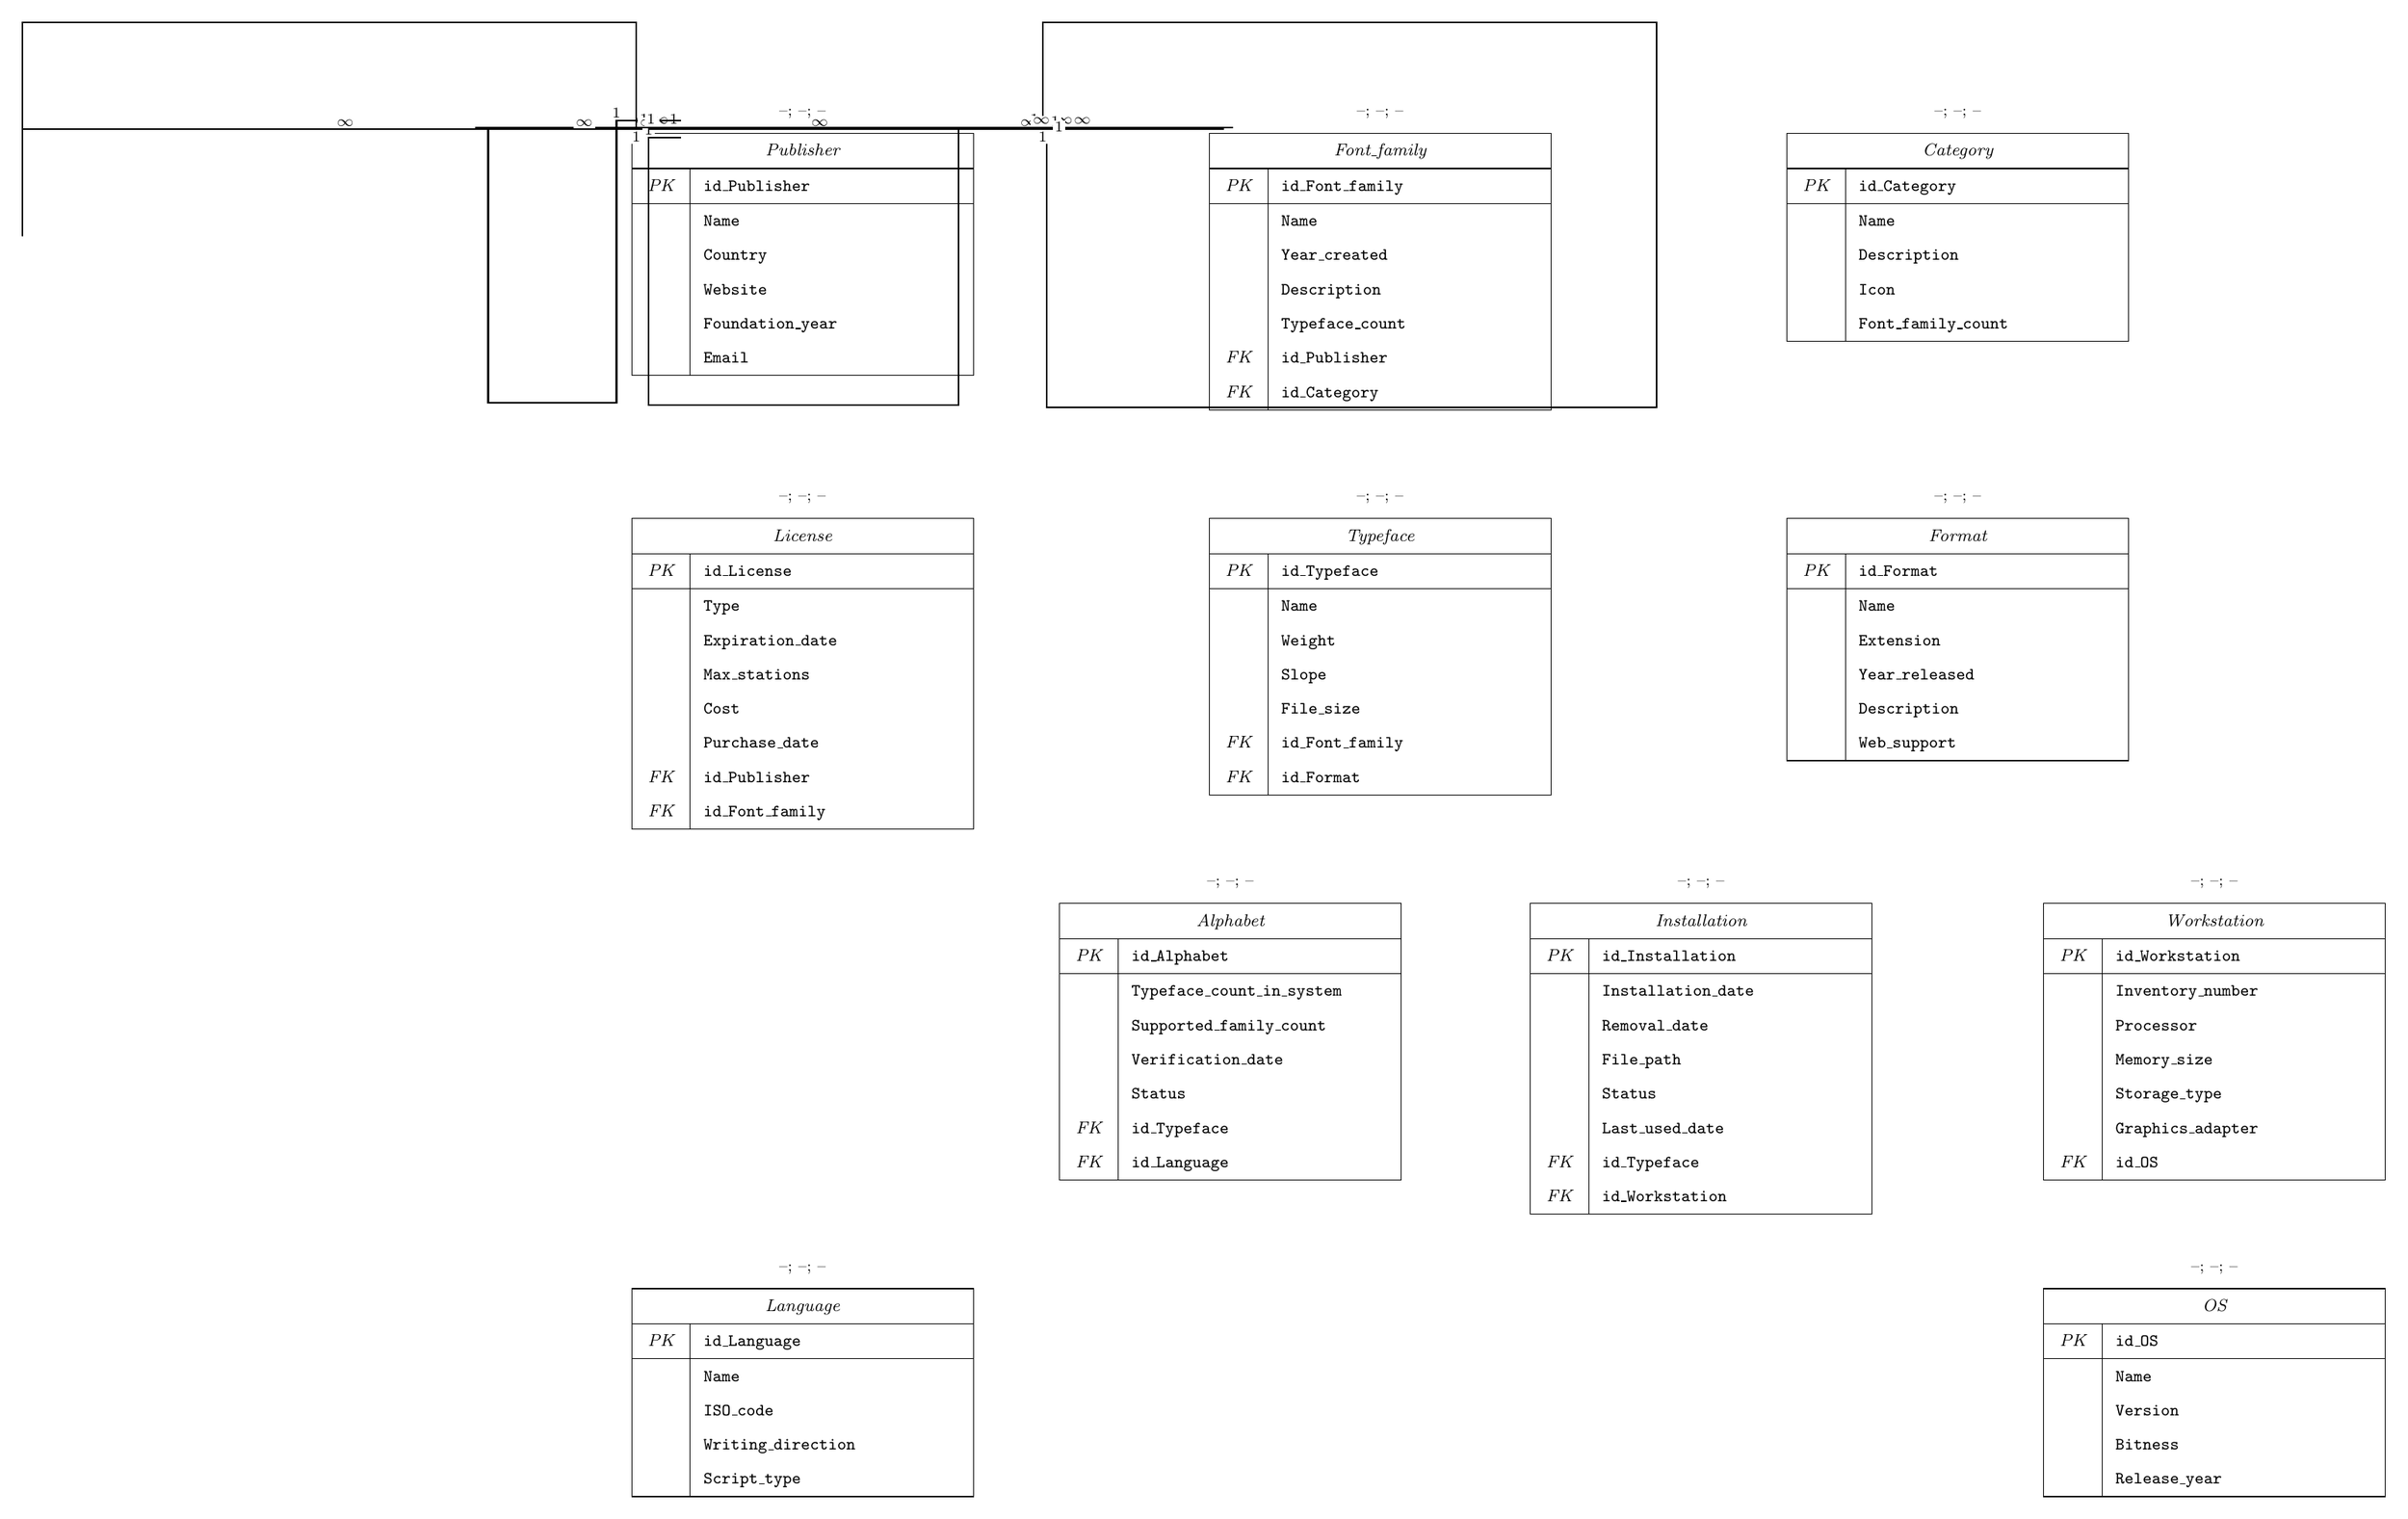
\begin{tikzpicture}[remember picture]

% === Row 1 ===

\def\tableVgap{18em}
\def\tableHgap{27em}

\dbtable{pub}{0,0}{
    \SetCell[c=2]{c} Publisher & \\
    PK & \tm{pub_pk}{id\_Publisher} \\
       & Name \\
       & Country \\
       & Website \\
       & Foundation\_year \\
       & Email \\
}
\node[ann, above=0.3em of pub] {--; --; --};

\dbtable{ff}{\tableHgap,0}{
    \SetCell[c=2]{c} Font\_family & \\
    PK & \tm{ff_pk}{id\_Font\_family} \\
       & Name \\
       & Year\_created \\
       & Description \\
       & Typeface\_count \\
    FK & \tm{ff_fk_pub}{id\_Publisher} \\
    FK & \tm{ff_fk_cat}{id\_Category} \\
}
\node[ann, above=0.3em of ff] {--; --; --};

\dbtable{cat}{\tableHgap * 2,0}{
    \SetCell[c=2]{c} Category & \\
    PK & \tm{cat_pk}{id\_Category} \\
       & Name \\
       & Description \\
       & Icon \\
       & Font\_family\_count \\
}
\node[ann, above=0.3em of cat] {--; --; --};

% === Row 2 ===

\dbtable{lic}{0,-18em}{
    \SetCell[c=2]{c} License & \\
    PK & \tm{lic_pk}{id\_License} \\
       & Type \\
       & Expiration\_date \\
       & Max\_stations \\
       & Cost \\
       & Purchase\_date \\
    FK & \tm{lic_fk_pub}{id\_Publisher} \\
    FK & \tm{lic_fk_ff}{id\_Font\_family} \\
}
\node[ann, above=0.3em of lic] {--; --; --};

\dbtable{tf}{\tableHgap,-18em}{
    \SetCell[c=2]{c} Typeface & \\
    PK & \tm{tf_pk}{id\_Typeface} \\
       & Name \\
       & Weight \\
       & Slope \\
       & File\_size \\
    FK & \tm{tf_fk_ff}{id\_Font\_family} \\
    FK & \tm{tf_fk_fmt}{id\_Format} \\
}
\node[ann, above=0.3em of tf] {--; --; --};

\dbtable{fmt}{\tableHgap * 2,-18em}{
    \SetCell[c=2]{c} Format & \\
    PK & \tm{fmt_pk}{id\_Format} \\
       & Name \\
       & Extension \\
       & Year\_released \\
       & Description \\
       & Web\_support \\
}
\node[ann, above=0.3em of fmt] {--; --; --};

% === Row 3 ===

\dbtable{lang}{0,-54em}{
    \SetCell[c=2]{c} Language & \\
    PK & \tm{lang_pk}{id\_Language} \\
       & Name \\
       & ISO\_code \\
       & Writing\_direction \\
       & Script\_type \\
}
\node[ann, above=0.3em of lang] {--; --; --};

\dbtable{alph}{20em,-36em}{
    \SetCell[c=2]{c} Alphabet & \\
    PK & \tm{alph_pk}{id\_Alphabet} \\
       & Typeface\_count\_in\_system \\
       & Supported\_family\_count \\
       & Verification\_date \\
       & Status \\
    FK & \tm{alph_fk_tf}{id\_Typeface} \\
    FK & \tm{alph_fk_lang}{id\_Language} \\
}
\node[ann, above=0.3em of alph] {--; --; --};

\dbtable{inst}{42em,-36em}{
    \SetCell[c=2]{c} Installation & \\
    PK & \tm{inst_pk}{id\_Installation} \\
       & Installation\_date \\
       & Removal\_date \\
       & File\_path \\
       & Status \\
       & Last\_used\_date \\
    FK & \tm{inst_fk_tf}{id\_Typeface} \\
    FK & \tm{inst_fk_ws}{id\_Workstation} \\
}
\node[ann, above=0.3em of inst] {--; --; --};

\dbtable{ws}{66em,-36em}{
    \SetCell[c=2]{c} Workstation & \\
    PK & \tm{ws_pk}{id\_Workstation} \\
       & Inventory\_number \\
       & Processor \\
       & Memory\_size \\
       & Storage\_type \\
       & Graphics\_adapter \\
    FK & \tm{ws_fk_os}{id\_OS} \\
}
\node[ann, above=0.3em of ws] {--; --; --};

\dbtable{os}{66em,-54em}{
    \SetCell[c=2]{c} OS & \\
    PK & \tm{os_pk}{id\_OS} \\
       & Name \\
       & Version \\
       & Bitness \\
       & Release\_year \\
}
\node[ann, above=0.3em of os] {--; --; --};

% ==================== LINKS ====================

\def\hgap{1.5em}
\def\xWestShift{-3.4em}
\def\xEastShift{12.6em}
\def\oneRowTablesLinkMargin{7.9em}

% Font_family.id_Publisher -> Publisher.id_Publisher
\draw[lnk] ([xshift=\xWestShift]ff_fk_pub.west) -- ++(-\hgap,0) node[crd, above] {$\infty$}
    |- ++(-\oneRowTablesLinkMargin, 0)
    |- ([xshift={\hgap + \xEastShift}]pub_pk.west)
    -- node[crd, above] {1} ([xshift=\xEastShift]pub_pk.west);

% Font_family.id_Category -> Category.id_Category
\draw[lnk] ([xshift=\xEastShift]ff_fk_cat.west) -- ++(\hgap,0) node[crd, above] {$\infty$}
    |- ++(\oneRowTablesLinkMargin, 0)
    |- ([xshift={-\hgap + \xWestShift}]cat_pk.west)
    -- node[crd, above] {1} ([xshift=\xWestShift]cat_pk.west);

% Font_family.id_Font_family -> Typeface.id_Font_family
\draw[lnk] ([xshift=\xEastShift]ff_pk.west) -- ++(\hgap,0) node[crd, below] {1}
    |- ++(0, 5em) |- ++(28.7em, 0) |- ++(0, -18em) |- ++(-28.5em, 0)
    |- node[crd, pos=0.75, above] {$\infty$} ([xshift=\xEastShift]tf_fk_ff.west);

% Publisher.id_Publisher -> License.id_Publisher
\draw[lnk] ([xshift=\xWestShift]pub_pk.west) -- ++(-\hgap,0) node[crd, above] {1}
    |- node[crd, pos=0.75, above] {$\infty$} ([xshift=\xWestShift]lic_fk_pub.west);

% Font_family.id_Font_family -> License.id_Font_family
\draw[lnk] ([xshift=\xWestShift]ff_pk.west) -- ++(-\hgap,0) node[crd, below] {1} |- ++(0, 5em) |- ++(-28.7em, 0) |- ++(0, -10em)
    |- node[crd, pos=0.75, above] {$\infty$} ([xshift=\xWestShift]lic_fk_ff.west);

% Typeface.id_Format -> Format.id_Format
\draw[lnk] ([xshift=\xEastShift]tf_fk_fmt.west) -- ++(\hgap,0) node[crd, above] {$\infty$}
    |- ++(\oneRowTablesLinkMargin, 0)
    |- ([xshift={-\hgap + \xWestShift}]fmt_pk.west)
    -- node[crd, above] {1} ([xshift=\xWestShift]fmt_pk.west);

% Typeface.id_Typeface -> Alphabet.id_Typeface
\draw[lnk] ([xshift=\xWestShift, yshift=.4em]tf_pk.west) -- ++(-\hgap*2,0) node[crd, above] {1}
    |- ++(0, -13.2em) |- ++(-6em, 0)
    |- node[crd, pos=0.75, above] {$\infty$} ([xshift=\xWestShift]alph_fk_tf.west);

% Typeface.id_Typeface -> Installation.id_Typeface
\draw[lnk] ([xshift=\xWestShift, yshift=-.4em]tf_pk.west) -- ++(-\hgap,0) node[crd, above] {1}
    |- ++(0, -12.5em) |- ++(14.5em, 0)
    |- node[crd, pos=0.75, above] {$\infty$} ([xshift=\xWestShift]inst_fk_tf.west);

% Alphabet.id_Language -> Language.id_Language
\draw[lnk] ([xshift=\xWestShift]alph_fk_lang.west) -- ++(-\hgap,0) node[crd, above] {$\infty$}
    |- ([xshift={\hgap + \xEastShift}]lang_pk.west)
    |- node[crd, above] {1} ([xshift=\xEastShift]lang_pk.west);

% Installation.id_Workstation -> Workstation.id_Workstation
\draw[lnk] ([xshift=\xEastShift]inst_fk_ws.west) -- ++(\hgap,0) node[crd, above] {$\infty$}
    |- ++(4.7em, 0)
    |- ([xshift={-\hgap + \xWestShift}]ws_pk.west)
    -- node[crd, above] {1} ([xshift=\xWestShift]ws_pk.west);

% Workstation.id_OS -> OS.id_OS
\draw[lnk] ([xshift=\xEastShift]ws_fk_os.west) -- ++(\hgap,0) node[crd, above] {$\infty$}
    |- node[crd, left, pos=0.75] {1} ([xshift=\xEastShift]os_pk.west);

\end{tikzpicture}
\caption{Database schema in English}
\end{figure}
\end{document}
